
\begin{figure}
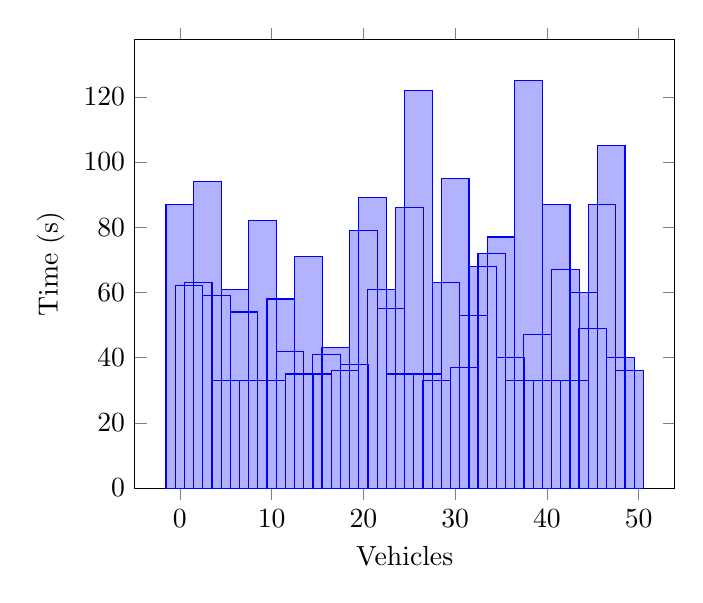
\begin{tikzpicture}
\begin{axis}[
legend style={anchor=west},
xlabel=Vehicles,
ylabel=Time (s),
ymin=0,
ybar,
]
\addplot coordinates {
(0, 87)
(1, 62)
(2, 63)
(3, 94)
(4, 59)
(5, 33)
(6, 61)
(7, 54)
(8, 33)
(9, 82)
(10, 33)
(11, 58)
(12, 42)
(13, 35)
(14, 71)
(15, 35)
(16, 41)
(17, 43)
(18, 36)
(19, 38)
(20, 79)
(21, 89)
(22, 61)
(23, 55)
(24, 35)
(25, 86)
(26, 122)
(27, 35)
(28, 33)
(29, 63)
(30, 95)
(31, 37)
(32, 53)
(33, 68)
(34, 72)
(35, 77)
(36, 40)
(37, 33)
(38, 125)
(39, 47)
(40, 33)
(41, 87)
(42, 67)
(43, 33)
(44, 60)
(45, 49)
(46, 87)
(47, 105)
(48, 40)
(49, 36)
};

\end{axis}
\end{tikzpicture}
\label{tik:100:90}
\caption{100 percent diving with GSC on route $90$}
\end{figure}
